\documentclass{beamer}
\usepackage{subfig}
\usepackage{amsmath}
\usepackage{bm}

\DeclareMathOperator*{\argmax}{arg\,max}
\DeclareMathOperator*{\argmin}{arg\,min}

\setbeamertemplate{footline}[frame number]
\title{Regularization and Model Selection}
\author{Prof. Alessandro Lucantonio}
\institute{Aarhus University}
\date{}

\setbeamertemplate{navigation symbols}{}

\begin{document}
	\frame{\titlepage}
	
		\begin{frame}
		\frametitle{Underfitting and overfitting - intuition}
		
		Imagine that you have to study for a written exam consisting of exercises. 
		
		\vspace{5mm}
		
		Doing only a few exercises while studying leads to poor perfomance both on homework and at the exam. This is called \textsl{underfitting}: the performance at the exam will be bad because of poor training.
		
		\vspace{5mm}
		
		Moreover, memorize all the solutions to homework leads to the maximum score on homework (trivially) but probably a bad score on the exam exercises. This is called \textsl{overfitting}: you have a bad performance on the exam because you did not capture the true essence of the homework, rather you have memorized their peculiarities.
	\end{frame}
	
	\begin{frame}
		\frametitle{Underfitting and overfitting - analytical example}
		\begin{figure}
			\centering
			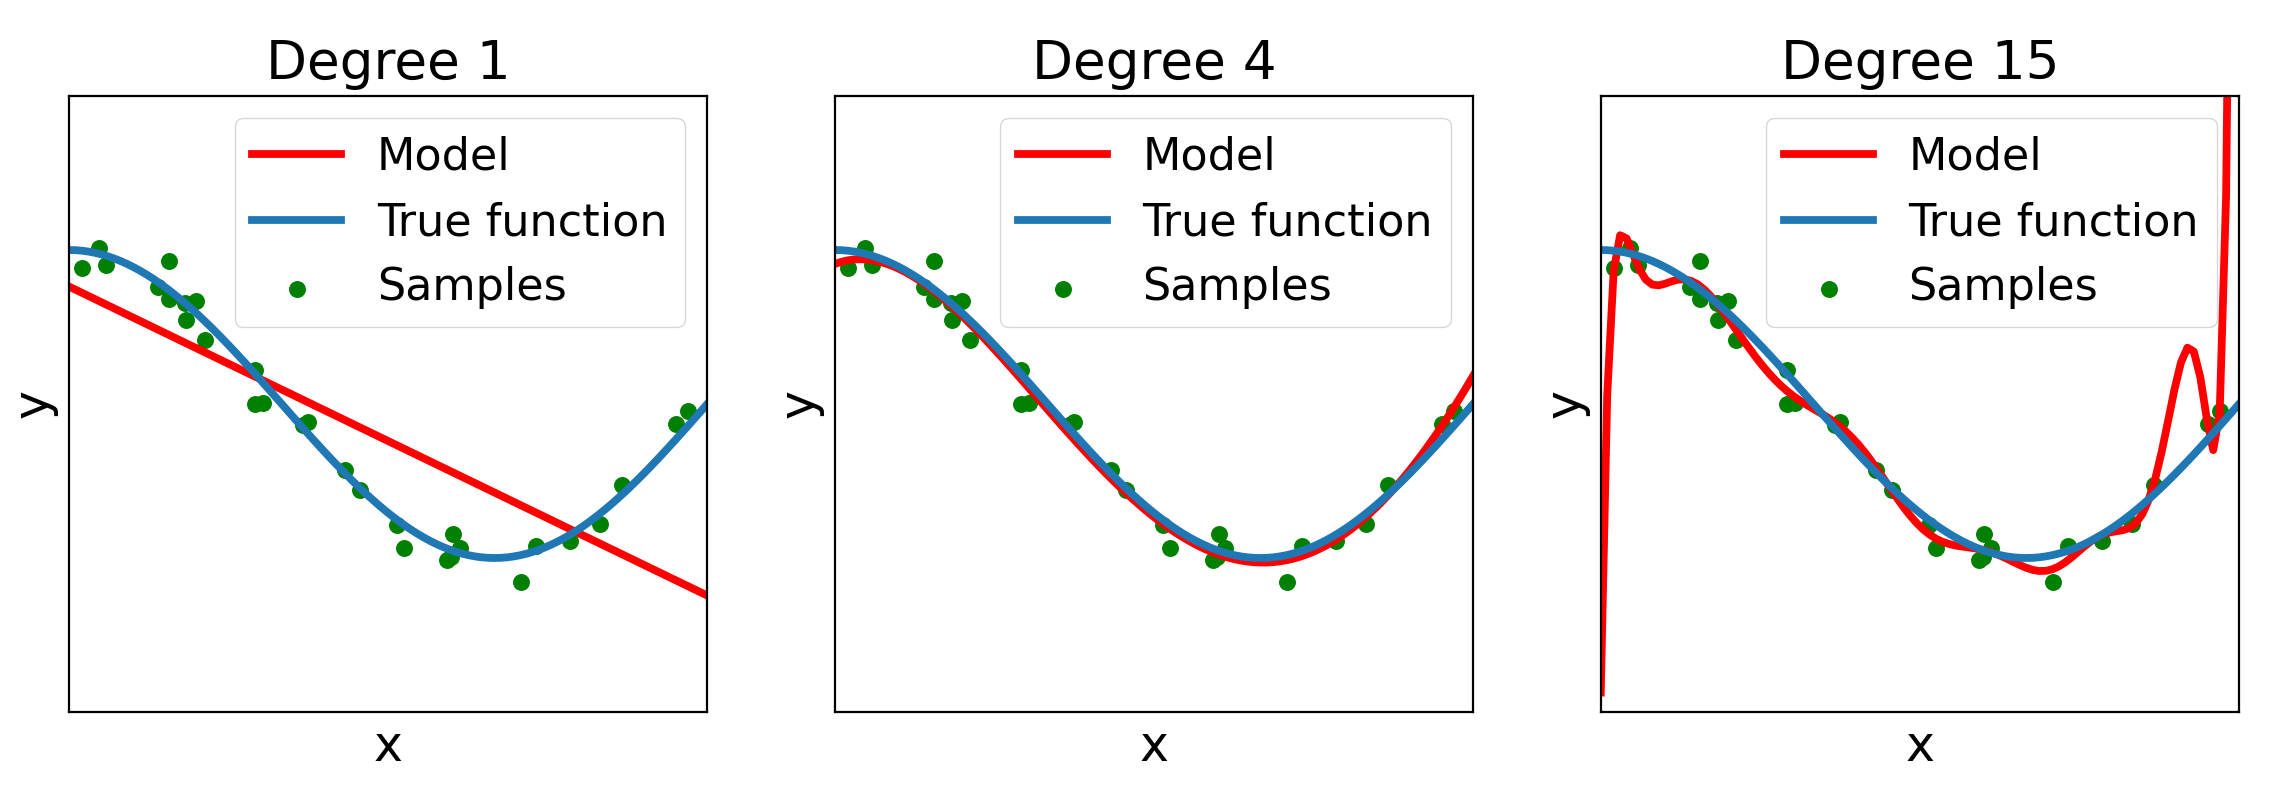
\includegraphics[scale=0.35]{images/overfitting_poly}
			\caption{Underfitting (polynomial degree 1), good fitting (polynomial degree 4), overfitting (polynomial degree 15).}
		\end{figure}
		
		Overfitting can be countered through:
		\begin{itemize}
			\item regularization;
			\item validation.
		\end{itemize}
	\end{frame}
	
	
	\begin{frame}
		\frametitle{Regularization}
		
		Overfitting is correlated with ``complex" models: to avoid them, we penalize models with large weights. One way to do this is to consider the following cost function
		\begin{equation*}
			E_{r}(\bm{w}) = E(\bm{w}) + R_{\lambda}(\bm{w})
		\end{equation*}
		where $R_{\lambda}$ is the \textsl{regularization term}. $\lambda > 0$ is a hyperparameter that must be chosen in the \textbf{model selection phase} (see later).
		
		\vspace{5mm}
		
		Most common regularization techniques:
		\begin{itemize}
			\item Tikhonov (or $L^2$ or \textit{Ridge}): $R_{\lambda}(\bm{w}) = \lambda ||\bm{w}||^2_2 = \lambda \sum_i w_i^2$. Tends to make \textit{all} weights small.
			\item LASSO (or $L^1$): $R_{\lambda}(\bm{w}) = \lambda ||\bm{w}||_1 = \lambda \sum_i |w_i|$. Tends to make \textit{some} weights $0$ (feature selection).
		\end{itemize}
	\end{frame}
	
	\begin{frame}
		\frametitle{Linear Regression with Tikhonov regularization}
		\begin{itemize}
			\item Cost function (without regularization):
			\begin{equation*}
				E(\bm{w}) = \frac{1}{N} ||\mathsf{X} \bm{w} - \bm{y}||^2
			\end{equation*}
			\item Regularized cost function:
			\begin{equation*}
				E_{r}(\bm{w}) = E(\bm{w}) + \lambda ||\bm{w}||^2
			\end{equation*}
			\item Gradient of the regularized cost function:
			\begin{equation*}
				\nabla E_r(\bm{w}) = \nabla E(\bm{w}) + 2 \lambda \bm{w} = 2\left(\frac{1}{N}\mathsf{X}^T(\mathsf{X}\bm{w} - \bm{y}) + \lambda \bm{w}\right)
			\end{equation*}
			\item Normal equation:
			\begin{equation*}
				\bm{w} = (\mathsf{X}^T\mathsf{X} + \lambda \mathsf{I})^{-1}\mathsf{X}^T\bm{y}
			\end{equation*}
			Note that in this case $\mathsf{X}^T\mathsf{X} + \lambda \mathsf{I}$ is \textsl{always} invertible (why?).
		\end{itemize}
		
		
	\end{frame}
	
\begin{frame}
	\frametitle{Bias-Variance trade-off}
	\textbf{Bias}: expected discrepancy between targets and predictions given by the model.
	
	\vspace{5mm}
	
	\textbf{Variance}: measure of the deviation from the expected value given by the model that any particular sampling of the data (from the same underlying data-generating distribution) is likely to cause.
	
	\vspace{5mm}
	
	Some intuitions on the effect of regularization:
	\begin{itemize}
		\item High $\lambda$ $\leadsto$ simple model $\leadsto$ high bias (underfitting).
		\item Low $\lambda$ $\leadsto$  complex model $\leadsto$  high variance (overfitting).
		\item Intermediate $\lambda$: optimal solution (good bias-variance trade-off).
	\end{itemize}
%	\begin{figure}
%		\centering
%		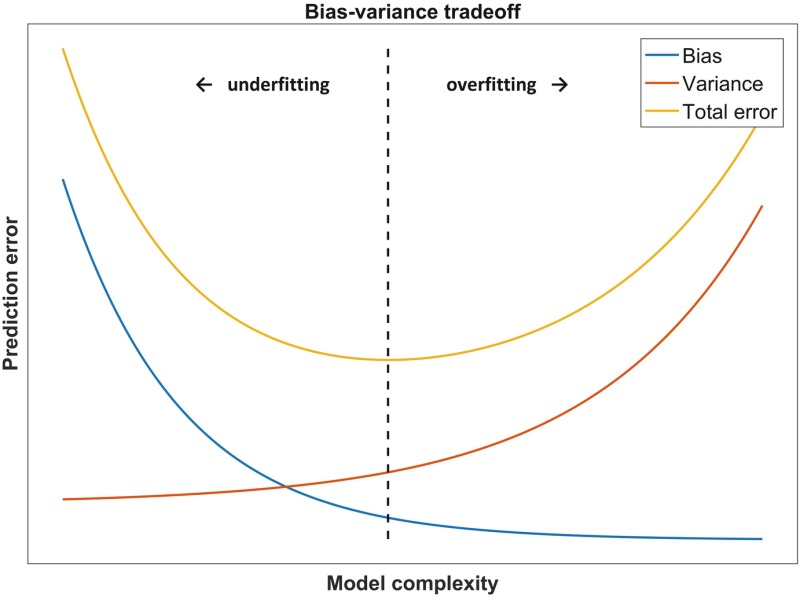
\includegraphics[scale=0.3]{images/bias-variance}
%		%\caption{Yellow curve: validation error.}
%	\end{figure}
\end{frame}
	
	\begin{frame}
		\frametitle{Generalization}
		Central challenge in Machine Learning: \textbf{generalization}! Our algorithm must perform well on \textit{new, previously unseen} inputs.
		
		\vspace{5mm}
		
		Recall that we have to find a balance between bias and variance. Even if we limit the complexity of our model using regularization, the training set does not provide a good estimate of the test (generalization) error.
		
		\vspace{5mm}
		
		In other words, generalization is compromised if we choose hyperparameters (including the regularization factor) only according to the training error.
	\end{frame}

	\begin{frame}
	\frametitle{Generalization - Training vs test error}
	\begin{figure}
		\centering
		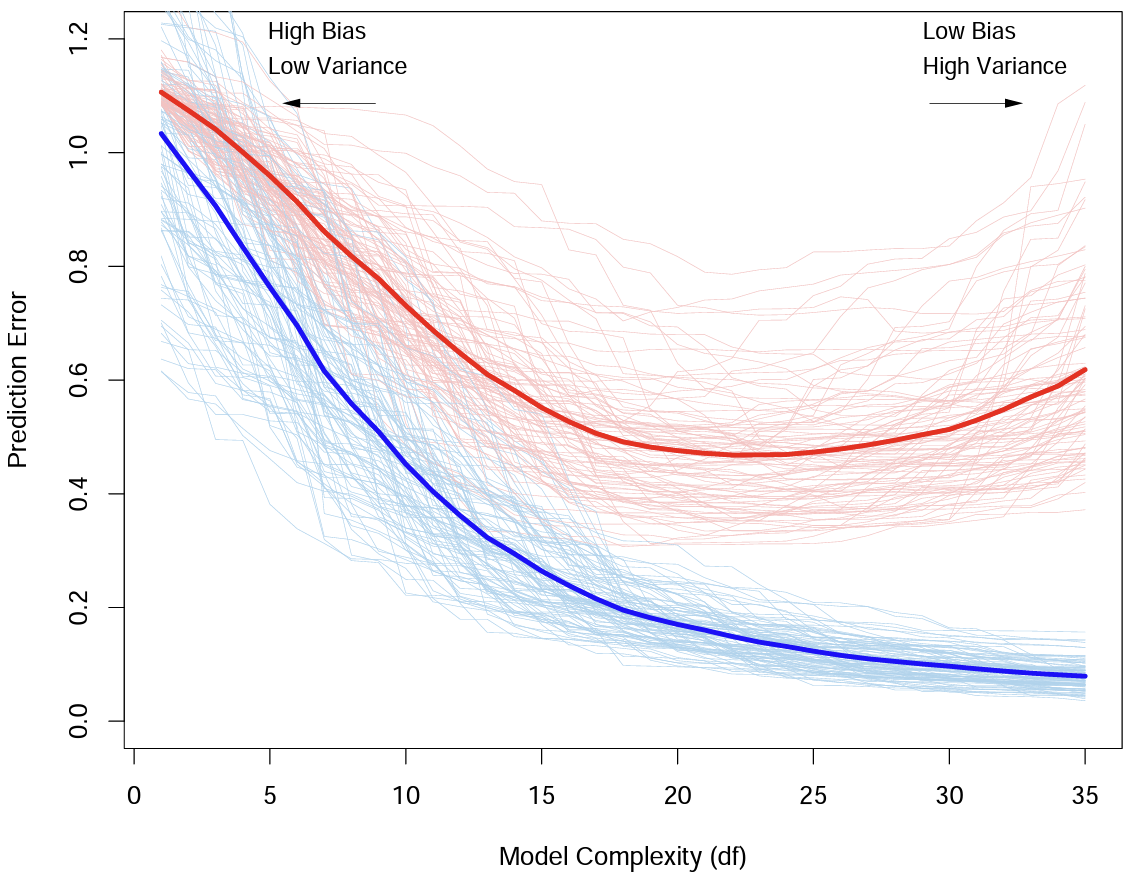
\includegraphics[scale=0.8]{images/model_selection_general_idea}
		\caption{Training (blue) and test (red) errors as the model complexity varies.}
	\end{figure}
\end{frame}

	\begin{frame}
	\frametitle{Early stopping}
	\begin{itemize}
		\item Store a copy of the model parameters every epoch the validation loss improves;
		\item if the validation loss does not improve for a fixed number of epochs (\textit{patience}), terminate and return the best parameters.
	\end{itemize}
	\begin{figure}
		\centering
		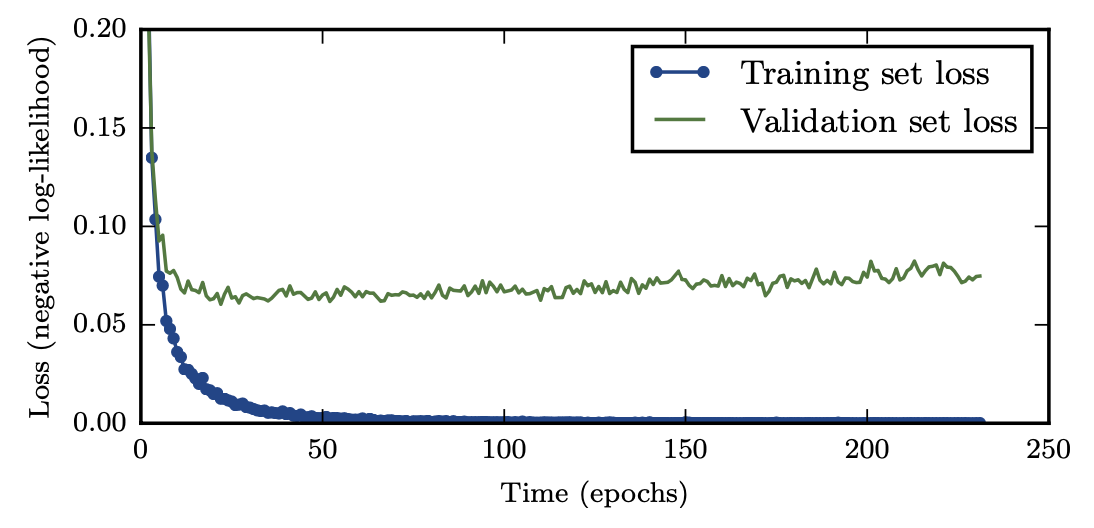
\includegraphics[scale=0.45]{images/early_stopping}
		\caption{Learning curves for a classifier trained on the MNIST dataset.}
	\end{figure}
\end{frame}

	\begin{frame}
		\frametitle{Model selection and model assessment}
		
		Do \textbf{not} use the test set to tune hyperparameters: introduce the \textbf{validation set}.
		
		\vspace{5mm}
		
		In general, we should distinguish between:
		\begin{enumerate}
		\item Model selection: estimate the performance of different models trained with different hyperparameters. 
		\item Model assessment: after choosing a final model we evaluate its performance on \textsl{new, previously unseen} (test) data.
		\end{enumerate}
		
		\vspace{5mm}
		
		Once we have selected a model using the validation set, we can assess its generalization error on the test set. Splitting the dataset into training and validation sets is called \textit{hold-out}.
	\end{frame}

	\begin{frame}
		\frametitle{Double Hold-out}
		\begin{figure}
			\centering
			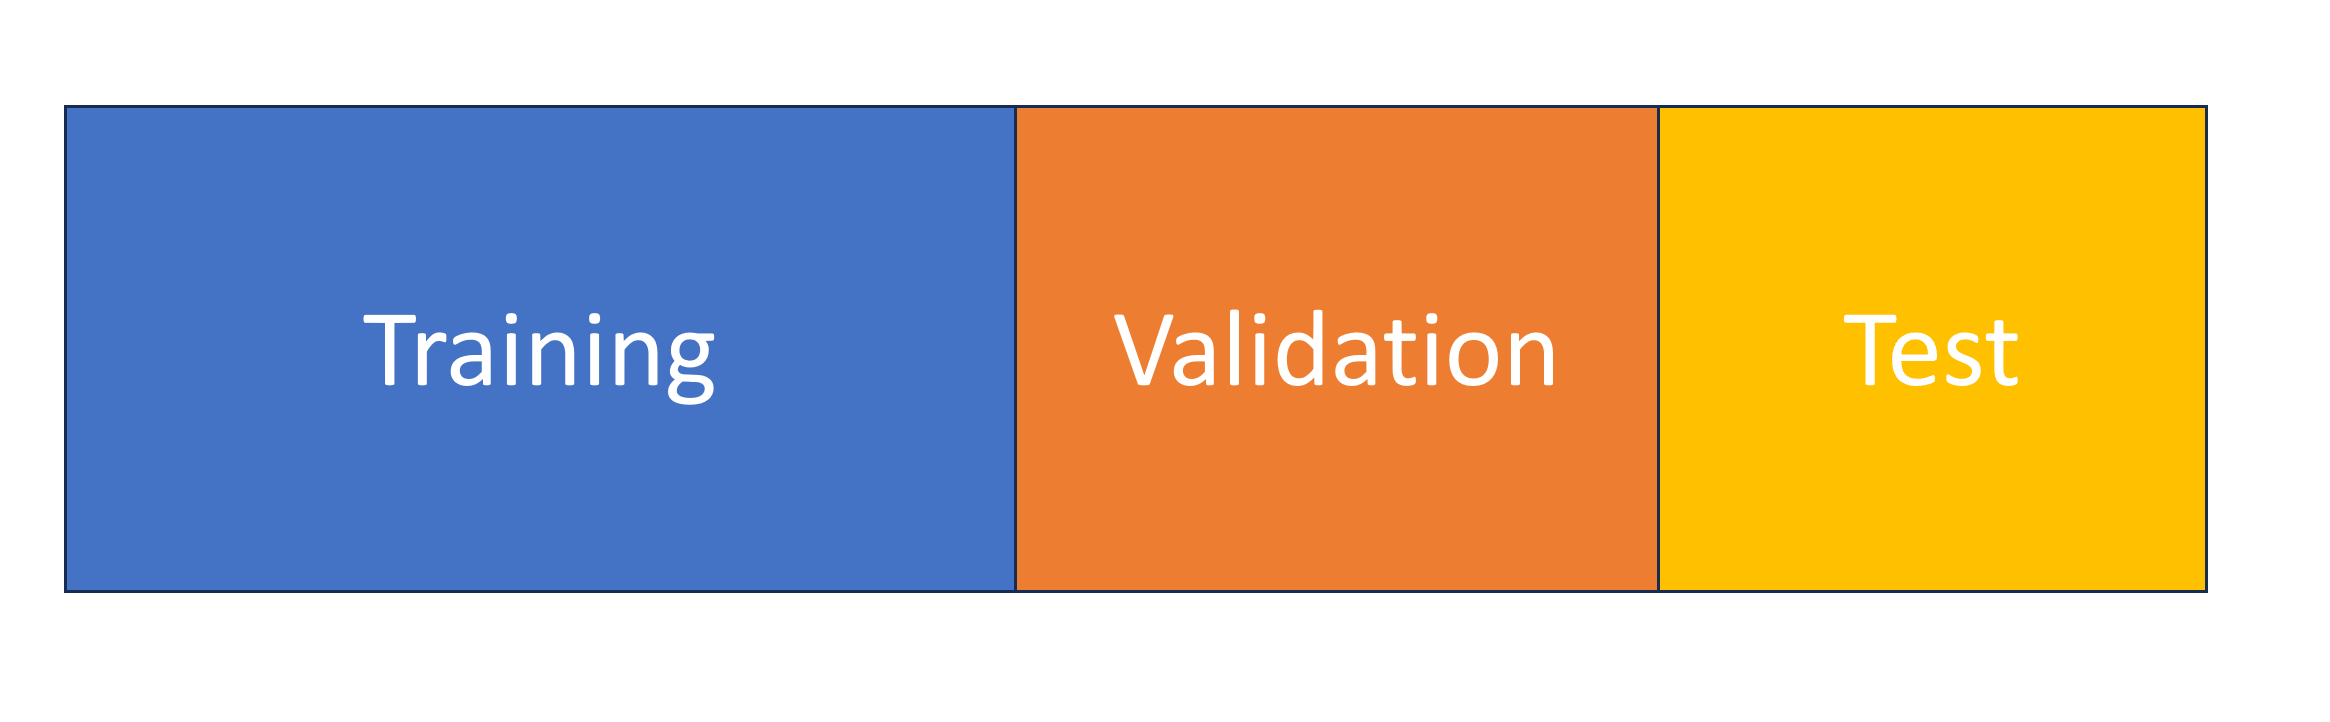
\includegraphics[scale=0.3]{images/hold-out}
		\end{figure}
		\begin{itemize}
			\item We split the entire dataset in three sets: training, validation and test (usually 60\%-20\%-20\% or  70\%-20\%-10\% of the total dataset). 
			\item Training set is used to fit the model. Then, we evaluate its validation performance and adjust its hyperparameters to maximize it. We re-fit the model and keep adjusting the hyperparameters until we find a model with a good trade-off between training and validation performance.
			\item We assess the generalization capability of the best model by evaluating the performance on the test set.
		\end{itemize}	
	\end{frame}

	\begin{frame}
		\frametitle{Cross-Validation}
		\begin{columns}
			\column{0.38\linewidth}
			\begin{figure}
				\centering
				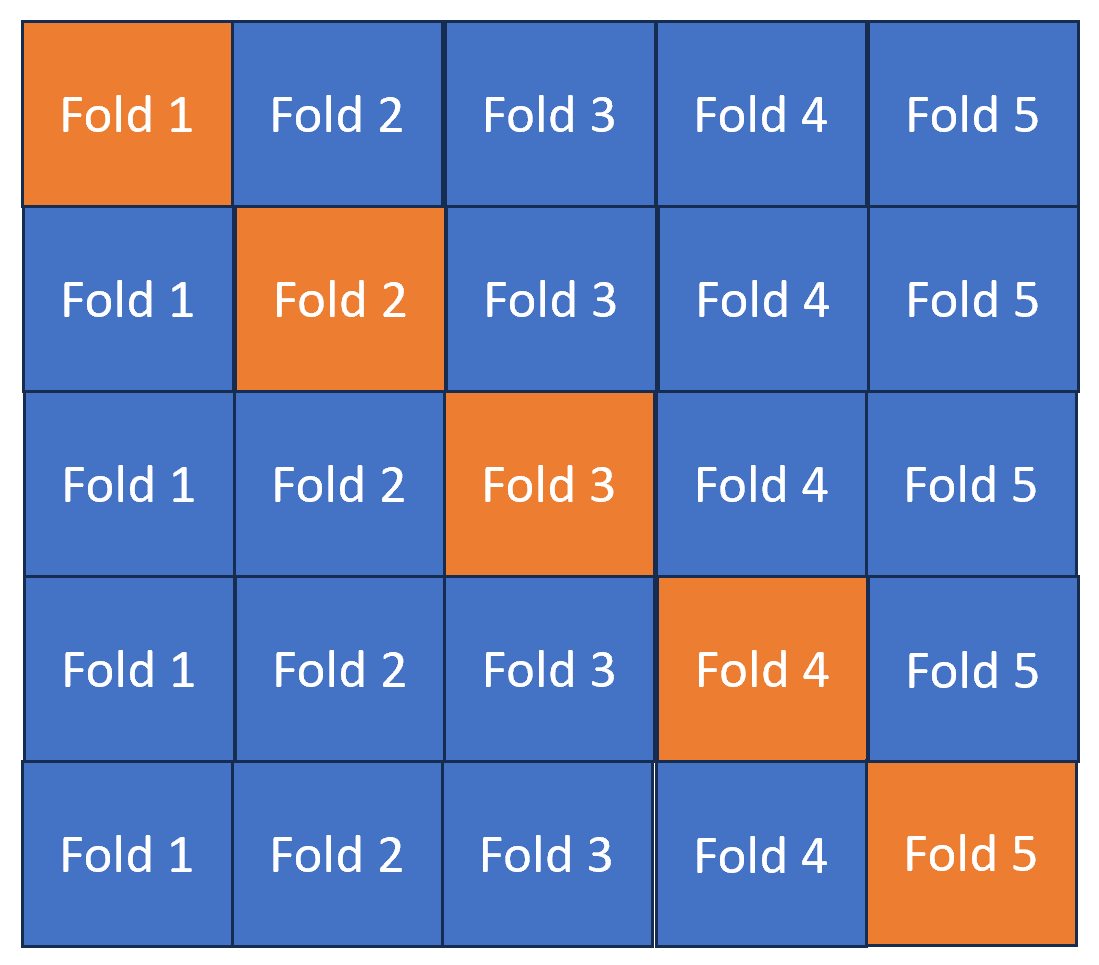
\includegraphics[scale=0.4]{images/cross-validation}
				\caption{5-fold CV}
			\end{figure}
			\column{0.58\linewidth}
			\begin{itemize}
				\item Split the data in $k$ disjoint \textit{folds}.
				\item Use $k-1$ folds as the training set and the remaining fold as the validation set. Repeat $k$ times (see figure).
				\item The performance will be the mean $\pm$ standard deviation computed across the $k$ runs.
			\end{itemize}
		\end{columns}
		
		\vspace{5mm}
		
		\textit{Pro}: Not sensitive to a particular partition of the data. Mean filter the error.
		
		\textit{Cons}: Computationally expensive (but parallellizable).
	\end{frame}

	\begin{frame}
		\frametitle{CV for selection and hold-out for assessment}
		\begin{enumerate}
			\item Split dataset into two sets (hold-out): development $D$ (model selection) and test $T$ (model assessment).
			\item Use the cross validation method on $D$ to select the best model.
			\textit{Optional}:  retrain the best model using the entire dataset $D$. 
			\item Evaluate the generalization error on the test set $T$.
		\end{enumerate}
	
	\end{frame}

	\begin{frame}
		\frametitle{Grid search}
		
		How to choose the best set of hyperparameters?
		
		\vspace{2mm}
		
		\textbf{Example}: two hyperparameters (learning rate $\alpha$ and regularization factor $\lambda$). Consider sets of three values for each parameter, e.g. $\alpha_{\text{vals}} = \{0.001, 0.01, 0.1\}, \lambda_{\text{vals}} = \{0.0001, 0.001, 0.01\}$. 
		
		Evaluate the model with $(\alpha, \lambda) = (i,j)$ for $i \in \alpha_{\text{vals}}, j \in \lambda_{\text{vals}}$.
		
		\begin{figure}
			\centering
			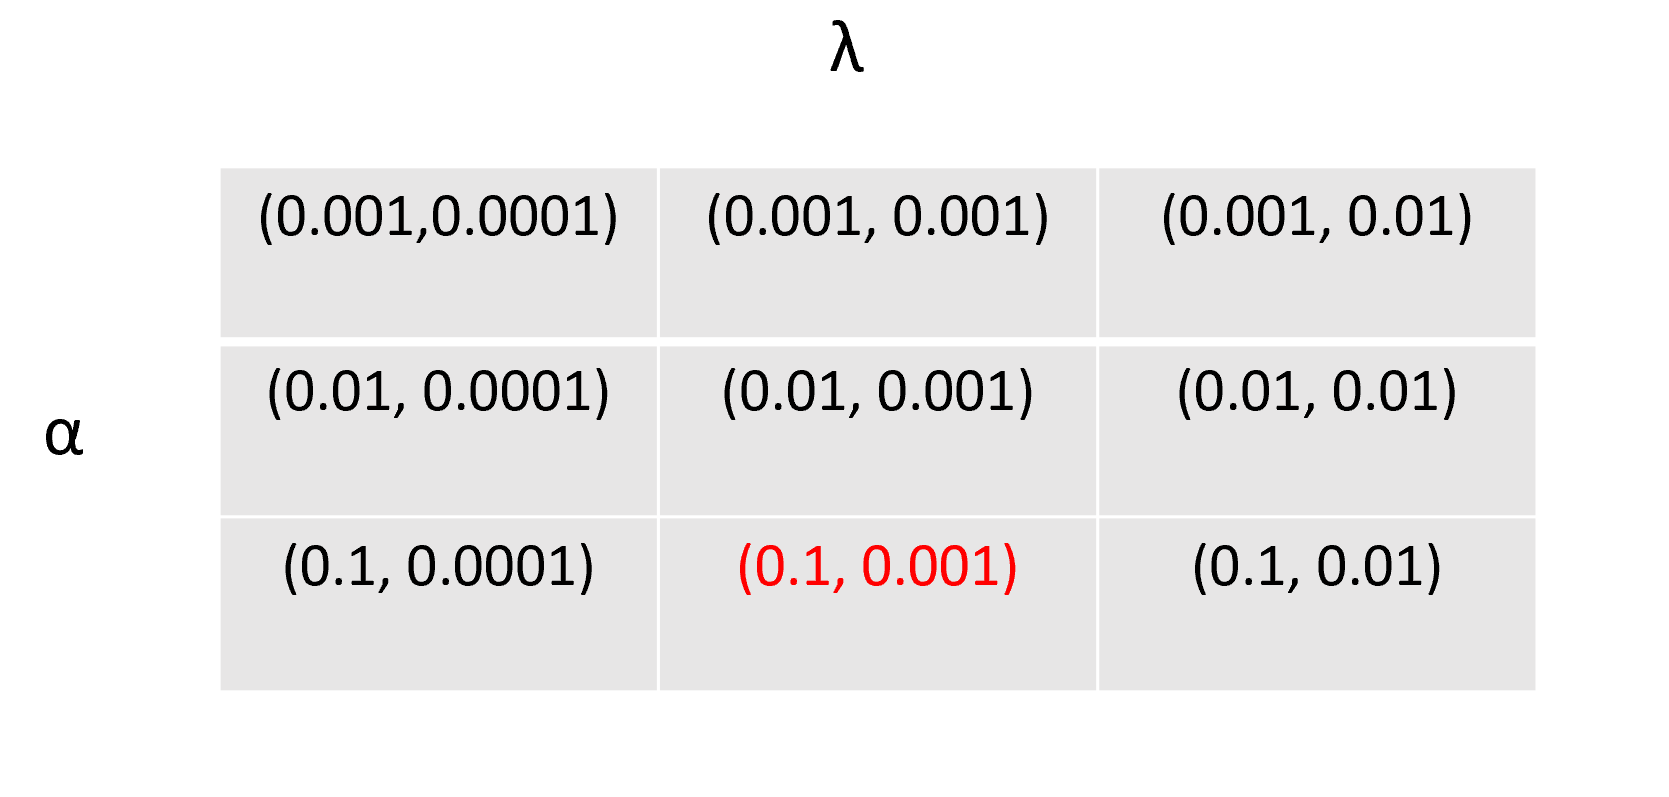
\includegraphics[scale=0.4]{images/grid-search}
		\end{figure}
		Choose the pair corresponding to the \textit{best performance on the validation set} (according, for example, to a $n$-fold CV). 
		
		\vspace{2mm}
		
		\textbf{Refinement}: Suppose that the best pair is $(0.1, 0.001)$. Then we can ``zoom in" and do another grid search with e.g. $\alpha_{\text{vals}} = \{0.075, 0.1, 0.125\}, \lambda_{\text{vals}} = \{0.00075, 0.001, 0.00125\}$. 
		
	\end{frame}
	
%	\begin{frame}
%		\frametitle{Effect of the training set size}
%		\begin{itemize}
%			\item With high \textbf{bias}: with large training set, training and validation errors will be high and close to each other. Increasing training set size (alone) will not help to reduce the validation error. 
%			\item With high \textbf{variance}:  with large training set, training error will increase while validation error will decrease without leveling off. Also, training error $<$ validation error but their difference remains significant. Increasing training set size is likely to help to improve the validation error.
%		\end{itemize}
%	\end{frame}

	
\end{document}